%
% File acl-hlt2011.tex
%
% Contact: gdzhou@suda.edu.cn
%%
%% Based on the style files for ACL2008 by Joakim Nivre and Noah Smith
%% and that of ACL2010 by Jing-Shin Chang and Philipp Koehn

\documentclass[11pt]{article}
\usepackage{acl-hlt2011}
\usepackage{times}
\usepackage{latexsym}
\usepackage{amsmath}
\usepackage{multirow}
\usepackage{url}
\usepackage{color}
\usepackage[vlined,figure]{algorithm2e}
\usepackage{graphicx} 

\DeclareMathOperator*{\argmax}{arg\,max}

\definecolor{red}{rgb}{1,0,0}

\newcommand{\mnote}[1]{\marginpar{%
  \vskip-\baselineskip
  \raggedright\footnotesize
  \itshape\hrule\smallskip\tiny{#1}\par\smallskip\hrule}}  

\newcommand{\mtodo}[1]{\mnote{\textcolor{red}{#1}}}
\newcommand{\todo}[1]{\textcolor{red}{TODO: #1}}
\newcommand{\secref}[1]{Section~\ref{#1}}
\newcommand{\tabref}[1]{Table~\ref{#1}}
\newcommand{\figref}[1]{Figure~\ref{#1}}
\newcommand{\code}[1]{{\small \tt #1}}
\newcommand{\emq}[1]{\emph{``#1''}}
\newcommand{\paraheader}[1]{\vskip 0.05in \noindent\emph{#1}}
\newcommand{\skipheader}{\vskip 0.05in}

\newcommand{\bm}{\boldsymbol}
\def\bs#1{\boldsymbol{#1}}

%\setlength\titlebox{6.5cm}    % Expanding the titlebox
\setlength\titlebox{3.75cm}    % Expanding the titlebox

\title{Toward Statistical Machine Translation without Parallel Corpora}

\author{}
%\author{Person\\
%  University of Awesome\\
%  Location\\
%  {\tt person@email}  \And
%  Person\\
%  University of Awesome\\
%  Location\\
%  {\tt  person@email}   \And
%  Person\\
%  University of Awesome\\
%  Location\\
%  {\tt  person@email}}

\date{}

\begin{document}
\maketitle
\begin{abstract}
The parameters of statistical translation models are typically estimated from bilingual parallel corpora.   In this paper we explore the idea of estimating the parameters of a phrase-based statistical machine translation system from monolingual corpora.  Existing research on inducing bilingual dictionaries from monolingual texts has largely focused on learning the translations of individual, high frequency words.   We extend the concept to estimate all the parameters of phrase-based translation: phrase translation pairs, lexical and phrasal translation probabilities, and re-ordering probabilities.  We begin with a fixed phrase-table and perform a feature lesion study that shows how much translation performance decreases when model parameters are removed, and how much of that loss can be restored when monolingually-estimated equivalents are added.  Overall, we show that over 70\% of the lost performance can be recovered with monolingual features alone.  Finally, we analyze challenges of inducing the phrase table from monolingual texts and suggest ways of pruning the search space.  
% Large volumes of parallel text are required before translation models produce high quality translations, but sufficiently large corpora are available for  very few language pairs.  On the other hand, monolingual data is widely available and cheap to collect.  In this work, we propose a set of cues derived from monolingual resources and systematically introduce them in a phrase-based machine translation pipeline \emph{in place} of features induced from parallel data.  We show on two language pairs that monolingual data can take us a long way toward  inducing a high quality machine translation system.

%The parameters of statistical translation models of are estimated from bilingual parallel corpora.    Large volumes of parallel text are required before translation models produce high quality translations, but sufficiently large corpora are available for  very few language pairs.  On the other hand, monolingual data is widely available and cheap to collect.  In this work, we propose a set of cues derived from monolingual resources and systematically introduce them in a phrase-based machine translation pipeline \emph{in place} of features induced from parallel data.  We show on two language pairs that monolingual data can take us a long way toward  inducing a high quality machine translation system.

%Current statistical machine translation methods rely on very large parallel corpora to achieve state of the art performance.  However, such resources are only available for very few language pairs as they are very expensive to obtain.  On the other hand, monolingual data (such as newswire) is widely available and cheap to collect.  In this work, we propose a set of cues derived from monolingual resources and systematically introduce them in a phrase-based machine translation pipeline \emph{in place} of features induced from parallel data.  We show on two language pairs that monolingual data can take us a long way toward  inducing a high quality machine translation system.\mtodo{Need a more concrete statement.}
\end{abstract}

% ------------------------------------------------

\section{Introduction} \label{sect:intro}

The parameters of statistical models of translation are typically estimated from bilingual parallel corpora \cite{Brown:1993}. 
In this work, we take an entirely different approach: we use monolingual resources to induce an end-to-end statistical machine translation system.  In particular, we extend a long line of work on inducing translation lexicons (beginning with \newcite{Rapp:1995}) to estimate all parameters for the phrase-based statistical machine translation \cite{Koehn:2003}.

Much of the prior work on lexicon induction is motivated by the idea that it could be applied to machine translation but stops short of actually doing so.  This work is a first attempt to extend and apply these ideas to an end-to-end machine translation pipeline. 
The promise of lexicon induction is that it could be used to create machine translation systems for languages which do not have extensive parallel corpora.  
Instead training would only require two large monolingual corpora and a small bilingual dictionary.
%, both of which are generally easy to obtain for a language.  
The idea is that monolingual distributional similarity and a handful of bilingual pairs to act as example mappings are enough to learn translations, because words behave similarly across languages.  Here we examine an idealized case where the distribution of words across languages is identical, by taking the two sides of a parallel corpus and treating them as independent monolingual corpora by forgetting the sentence alignments. In this paper we:

%Current statistical machine translation (SMT) methods (e.g. \cite{Koehn:2003,Chiang:2005}) crucially rely on vast amounts of sentence aligned translations in order to achieve state of the art performance.  These resources are only available for very few language pairs because producing them in sufficient quantities is an expensive and time consuming endeavor.  Moreover, the SMT system performance tends to drop if test data comes from a different domain then the parallel data used in training\mtodo{Need a good MT adaptation reference}.  

%The rest of the paper is organized as follows.  \secref{sect:bckg} begins with the relevant background on the phrase-based SMT framework we will use in the rest of the paper and continues to give a brief overview of the existing work on inducing translation lexicons. \secref{sect:mono} motivates and introduces translation and reordering features induced from monolingual data alone.   \secref{sect:exp} studies the informativeness of these features as they are added to the Machine Translation pipeline.  Finally, \secref{sect:conc} concludes and discusses directions for future work.

\begin{itemize}
  \item Analyze the challenges of using bilingual lexicon induction for statistical machine translation (performance on low frequency items, moving from words to phrases, and dealing with prohibitively large search space).
  \item Extend bilingual lexicon induction to phrases, and scale it to extract translations of tens of thousands of  phrases (which naively requires trillions of phrase comparisons). 
  \item Perform a lesion study in which all feature functions are dropped from from a phrase table and then replaced with monolingually estimated equivalents.
  \item Propose a novel algorithm for estimating phrase reordering features from monolingual texts.
  \item Report end-to-end translation quality with (1) a fixed phrase-table with monolingually estimated parameters and (2) a phrase-table created without any sentence-aligned parallel data.
\end{itemize}

% ------------------------------------------------
\section{Related Work} \label{sect:related-work}

The first formulation of statistical machine translation (SMT) is due to the early work by~\newcite{Brown:1993} at IBM, which proposed a series of probabilistic models based on word-to-word correspondences.  The best performing current methods, so-called {\em phrase-based} and {\em hierarchical} models \cite{Och:2002,Koehn:2003,Chiang:2005} extend the build on the IBM models, treating multi token phrases as building blocks for producing new translations.  One significant problem with these models is that their parameters are estimated from large quantities of sentence aligned translations.  These parallel resources are only available for a small set of language pairs and are very expensive to compile in sufficient quantities.  In this work, we estimate the parameters of the phrase-based formalism (reviewed in \secref{sect:bckg:smt}) from {\em monolingual} texts, which are easy to collect online. \mtodo{Mention parallel data extraction work, e.g. Marku, Smith, Uszkoreit?}

Our methods for estimating model parameters from monolingual corpora build on the long line of work in lexicon induction. \newcite{Rapp:1995} was the first to propose using context of a given word as a clue to its translation.  The model populates a bilingual lexicon by using a small seed dictionary to project context vectors across two languages and score their similarity. \newcite{Rapp:1999}, and \newcite{Fung:1998} build on the original idea proposing alternative similarity metrics. \newcite{Schafer:2002} exploited the idea that word translations tend to co-occur in time across languages. \newcite{Klementiev:2006b} used this temporal cue to train a phonetic similarity model for associating Named Entities across languages.  \newcite{Koehn:2002} used similarity in spelling as another kind of cue that a pair of words may be translations of one another.  In this work, we extend these ideas to estimate three independent kinds of metrics to score {\em phrasal} translation candidates.  More recent work on lexical induction includes \newcite{Haghighi:2008} who made use of contextual and orthographic clues to learn a generative model from monolingual texts and a seed lexicon, and \newcite{Mimno:2009} who proposed a polylingual topic model and matched high probability words in each topic across languages.  While effective for a small number of topics, it is unlikely to scale well to large multilingual dictionaries.

%\todo{The following text is stolen from my CoNLL paper with Nikesh, we need to replace it or reshape it to be relevant}
%\todo{Make citations real}
%The idea of words with similar meaning having similar contexts in the same language comes from the Distributional Hypothesis (Harris, 1985) and Rapp (1999) was the first to propose using context of a given word as a clue to its translation. Given a German word with an unknown translation, a German context vector is constructed by counting its surrounding words in a monolingual German corpus.  Using an incomplete bilingual dictionary, the counts of the German context words with known translations are projected onto an English vector.  The projected vector for the German word is compared to the vectors constructed for all English words using a monolingual English corpus.  The English words with the highest vector similarity are treated as translation candidates.  The original work employed a relatively large bilingual dictionary containing approximately 16,000 words and tested only on a small collection of 100 manually selected nouns.

%Koehn and Knight (2002) tested this idea on a larger test set consisting of the 1000 most frequent words from a German-English lexicon. They also incorporated clues such as frequency and orthographic similarity in addition to context. Schafer and Yarowsky, (2002) independently proposed using frequency, orthographic similarity and also showed improvements using temporal and word-burstiness similarity measures, in addition to context. Haghighi et al., (2008) made use of contextual and orthographic clues for learning a generative model from monolingual corpora and a seed lexicon.


% ------------------------------------------------

\section{Background} \label{sect:bckg}
\subsection{Parameters of phrase-based SMT} \label{sect:bckg:smt}

We attempt to use monolingual texts and an incomplete bilingual dictionary to estimate the parameters of a phrase-based translation  model \cite{Koehn:2003,Moses}.  Phrase-based translation typically starts by word-aligning a bilingual parallel corpus \cite{Och2003}.  The viterbi word alignments determine the parameters of phrase-based SMT.  These parameters are:

\begin{itemize}
\item \emph{Phrase pairs}.  
Phrase extraction heuristics \cite{Venugopal2003,Tillmann2003,Och2004} produce a set of phrase pairs ${<e, f>}$ that are `consistent' with the word alignments.  We consider the inventory of phrase pairs (irrespective of their scores) to be a model parameter.  Monolingual parameter estimation must have a mechanism to create a similar inventory to be considered a phrase-based translation model.

\item \emph{Phrase translation probabilities}.  Each phrase pair has a list of associated feature functions.  These include phrase translation probabilities ${\phi(e|f)}$ and ${\phi(f|e)}$ which are  typically calculated using maximum likelihood estimation. 

\item \emph{Lexical weighting}.  Since MLE overestimates ${\phi}$, smoothing is done with lexical weighting.  The phrase pair internal word alignments are used to 

\item \emph{Reordering model}.  monotone, swap, and discontinous
See \figref{fig:reorderfeats}.
\cite{tillman:2004:HLTNAACL,Kumar2004}

\item \emph{Other features (not bilingually estimated)}. Language model, phrase penalties.
\end{itemize}

Log linear formulation:
  \begin{eqnarray*}
    p(\mathbf{e} | \mathbf{f}) & \propto & \exp \sum_{i=1}^{n}{\lambda_i h_i (\mathbf{e}, \mathbf{f})} \label{log-linear-formulation}\\
    \hat{e} & = & \argmax_{e}{p(\mathbf{e} | \mathbf{f}) }
  \end{eqnarray*}


\begin{figure}[t]
\vskip 0.1in
\begin{center}
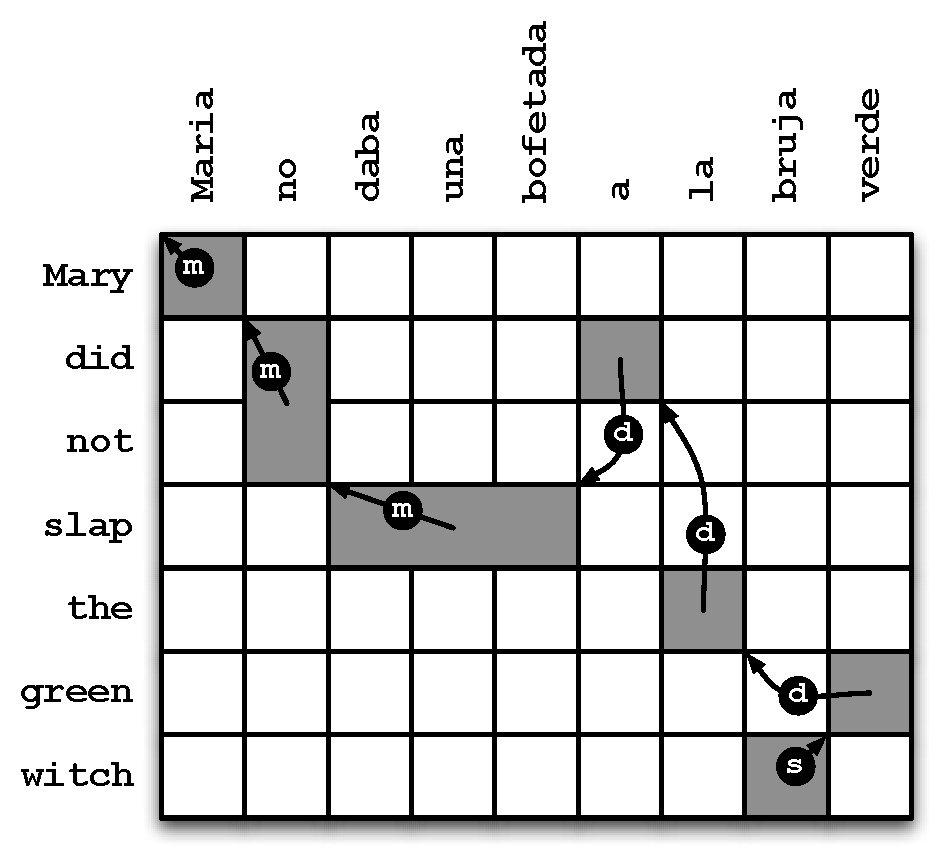
\includegraphics[width=0.8 \linewidth]{../figures/reorderfeats/reorderfeats.pdf}
\caption{Example alignment along with three kinds of orientations: monotone (m), swap (s), and discontinuous (d). }
\label{fig:reorderfeats} 
\end{center}
%\vskip -0.2in
\end{figure}

In this work, we will use the same general mathematical formulation, but propose alternative features derived directly from monolingual data.

 \subsection{Bilingual lexicon induction for SMT} \label{sect:bckg:lexind}
 
There are inherent challenges in extending lexicon induction methods to statistical machine translation.  

First, scaling these methods up substantially degrades their performance due to sparsity issues. High accuracy results reported in most of the previous literature on a small set of source language words (e.g. 100 nouns in \cite{Rapp:1995}, or 1,000 most frequent words in \cite{Koehn:2002}) tend to be misleading when the goal is to induce large translation dictionaries.  Figure \figref{fig:lexinduct} shows an experiment using English and Spanish Wikipedia articles and contextual similarity to rank candidate target words for 1,000 most frequent and 1,000 random source language tokens\footnote{These accuracy estimates are conservative, since only the translations present in our seed dictionary were counted.}.  Unsurprisingly, frequent terms have a substantially better chance of being paired up with the correct translation.  These concerns are exacerbated when we move to multi-token phrases.  As with phrase translation features estimated from parallel data, longer phrases are more sparse making similarity scores less reliable then they are for single words.  In \secref{sect:lexfeats}, we introduce additional similarity estimates less prone to sparsity issues.  In \secref{sect:exp:replacement} we show that monolingual features are very informative and reliable in our setting; even when added alongside the feature functions derived from parallel data, they account for over a BLEU point gain in performance.

\begin{figure}[t]
%\vskip 0.1in
\begin{center}
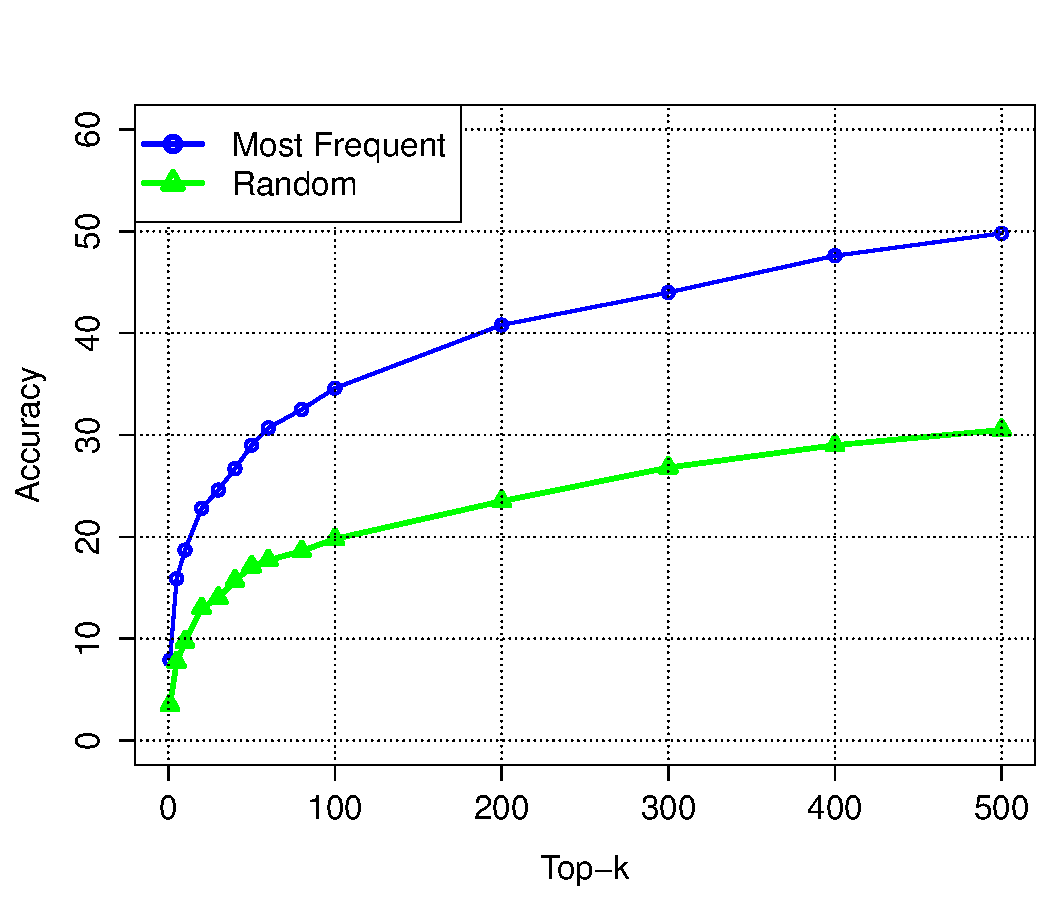
\includegraphics[width=\linewidth]{../figures/lexinduct/lexinduct.pdf}
\caption{Accuracy on English and Spanish Wikipedia articles for 1,000 most frequent and 1,000 random source words.  Accuracy is the proportion of the source words with at least one correct translation in the induced top-k list of candidates.}
\label{fig:lexinduct}
\end{center}
\vskip -0.2in
\end{figure}

Second, extending the bilingual lexicon induction methods to the induction of multi-word translation pairs greatly increases computational cost. Since each source-target pair must be scored, we would need to compute $|V_{f}| * |V_{e}|$ similarity scores, where $|V_{f}|$ and $|V_{e}|$ are the number of unique items in the source and target vocabularies. When we move from tokens to multi word phrases, $|V|$ grows to the number of unique {\it n}-grams. Exhaustively scoring all phrase pairs up to length three requires computing scores between the set of unique unigrams, bigrams and trigrams in the source and target languages.  In section \secref{sect:extract}, we propose methods to substantially reduce the number of comparisons, while keeping good translation candidates.

% ------------------------------------------------

\section{Monolingual Parameter Estimation} \label{sect:mono}

\subsection{Phrase scoring} \label{sect:score}

In place of phrase scores estimated from bilingual alignments, we propose similarity scores computed  from monolingual resources.  In this section, we introduce two kinds of scores we call {\em phrasal} and {\em lexical similarity} features.  The former score entire phrases, while the latter use word-level alignments between the phrase pairs to calculate lexical level scores.  The motivation is analogous to the two kinds of features we introduced in \secref{sect:bckg}: lexical similarity features are informative for rare phrases that have less reliable phrasal similarity scores because of sparse counts. 

\subsubsection{Phrasal similarity features} \label{sect:phrasalfeats}

\paraheader{Contextual similarity.}  We extend the vector space approach of \newcite{Rapp:1999} to compute similarity between \emph{phrases} in the source and target languages.  More formally, assume that $(s_{1}, s_{2}, \dots s_{N})$ and $(t_{1}, t_{2}, \dots t_{M})$ are (arbitrarily indexed) source and target vocabularies, respectively.  A source phrase $f$ is represented with an $N$ and target phrase $e$ with a $M$ dimensional vector (see \figref{fig:contextual}).  Only the components corresponding to words that appear in the context of a phrase in data take on non-zero values, which typically measure how ``unique'' a word is to the context in the dataset.  Next, $f$'s contextual vector is projected by mapping its components to the target space using the small number of word-word translations taken from a seed dictionary, but retaining the source component value.  Finally, the pair ($f, e$) is scored by computing similarity between the target  and projected source vectors.  Various means of computing the component values and vector similarity measures have been proposed in literature (e.g. \newcite{Rapp:1999,Fung:1998}).  We compute the value of the $k$-th component of $f$'s contextual vector  as follows: 

\begin{equation*}
w_{k} = n_{f,k} \times (log( {n / n_{k}}) + 1)
\end{equation*}

\noindent where $n_{f,k}$ and $n_{k}$ are the number of times $s_{k}$ appears in the context of $f$ and in the entire corpus, and $n$ is the maximum number of occurrences of any word in the data.  Intuitively, the more frequently $s_{k}$ appears with $f$ and the less common it is in the corpus in general, the higher its component value.  Similarity between two resulting vectors is measured as a cosine of the angle between them.

\begin{figure}[t]
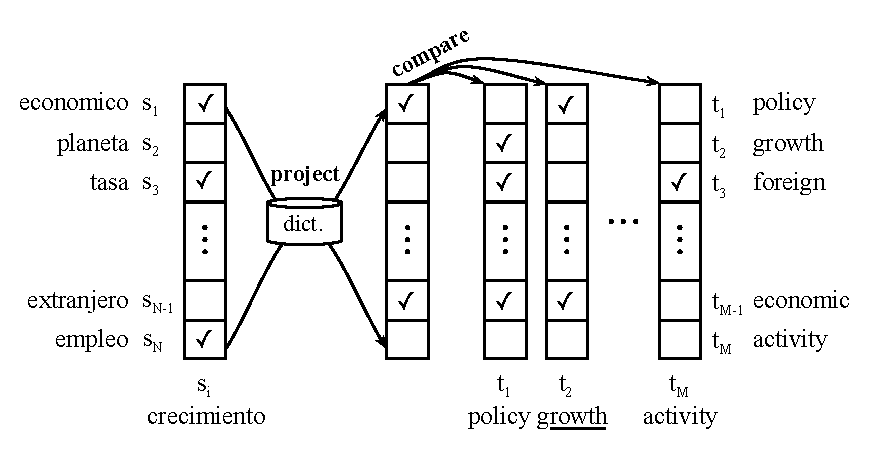
\includegraphics[width=\linewidth]{../figures/contextual/contextual}
\caption{Scoring contextual similarity: first, contextual vectors are projected using a small seed dictionary and then compared with the target language candidates.}
\label{fig:contextual}
\end{figure}

\mtodo{Give an example Spanish phrase and the English phrases that it has the highest similarity with}

\begin{figure}[t]
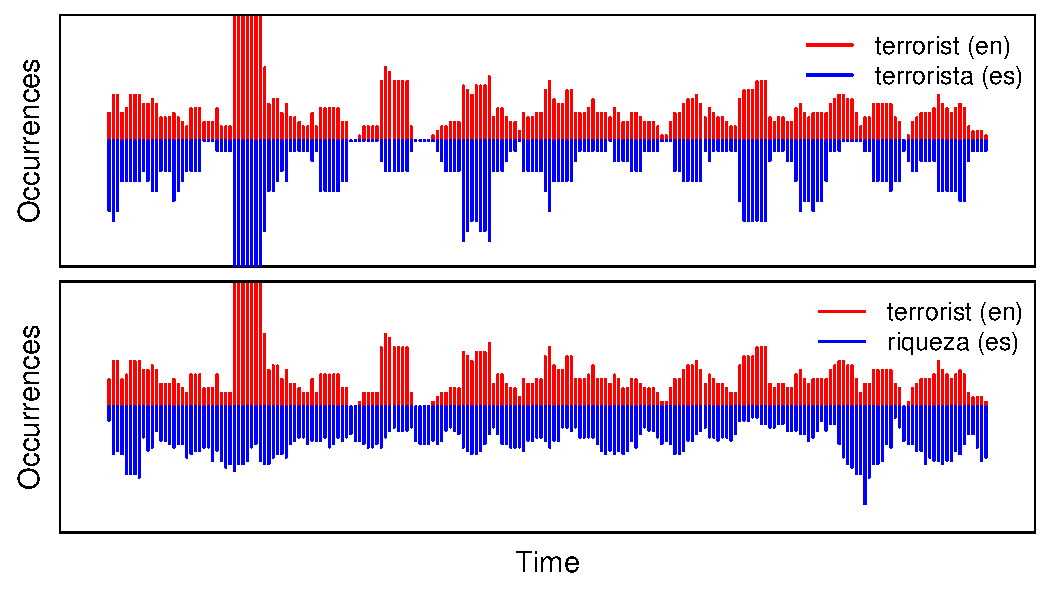
\includegraphics[width= \linewidth]{../figures/temporal/temporal}
\caption{Temporal histograms of the English word {\em terrorist}, its Spanish translation {\em terrorista}, and the words {\em ataques}  (attacks) and {\em riqueza} (wealth) collected from a subset of the Europarl corpus. While the correct translation has a better temporal match, the word {\em ataques} is often used around the same dates and shares a number of peaks of occurrences with the word {\em terrorist}.  The third word has a distinctly different temporal signature.}
\label{fig:temporal}
\end{figure}

\paraheader{Temporal similarity.} In addition to contextual similarity, words in two different languages may be scored in terms of their temporal similarity.  The intuition is that news stories from different countries will tend to discuss the same world events on the same day.  The frequencies of words over time give them particular signatures, that will tend to spike in on the dates across languages.  For instance, if the term {\it tsunami} is used frequently during a particular time span, the number of mentions of the Spanish word {\it maremoto} is very likely to increase in the same timeframe.     \figref{fig:temporal} illustrates how the temporal distribution of {\it terrorist} is more similar to the Spanish {\it terroista} than to other Spanish words.  This can be thought of as a weak signal that two phrases are translations of each other.  In order to score a pair of phrases across languages, we can compute the similarity of their temporal signatures. To generate a time sequence for a given word, we first sort the set of (time-stamped) documents of our corpus into a sequence of equally sized temporal bins.  We then count the number of occurrences of a phrase in each bin.  Following \newcite{Klementiev:2006b}, we use the cosine measure to score the temporal similarity of words by computing counts in a sliding window and normalizing the sequence. 

\mtodo{Give a couple of examples of phrase pairs that have high temporal similarity.  Possibly using the same example as for the contextual similarity.}

\mtodo{integrate citations to these two papers in this section: 
"lexical relationships from temporal patterns"
\cite{alfonseca-ciaramita-hall:2009:EMNLP}
Also
\cite{Schafer:2002}}

\subsubsection{Lexical similarity features}  \label{sect:lexfeats}

\paraheader{Contextual and Temporal similarity.}  Another way to estimate the quality of a phrasal translation is to score the similarity of individual words within the phrases.  To compute these lexical similarity features, we first average similarity scores (contextual or temporal) over all aligned words across the two phrases.  We then scale the score by the proportion of aligned words in the two phrases, effectively penalizing poorly aligned phrase pairs.\mtodo{Mention that it is the average of both forward and backward alignments?}

\paraheader{Orthographic / phonetic similarity.} Etymologically related words often retain similar spelling across languages with the same writing system, and the edit distance can be used to measure their similarity.  We use word alignments as before to score entire phrases for orthographic similarity.\mtodo{Not done quite the same as above but will glance over it.} We can also extend this idea to language pairs not sharing the same writing system, since many cognates and transliterated words remain phonetically similar.  Transliterations can be generated for tokens in a source phrase (e.g. \cite{Virga:2003}), with phrase similarity computed as before.

\skipheader In our experiments in \secref{sect:exp}, we will focus on the similarity scores introduced in this section.  However, note that various other similarity scores\mtodo{list them} can be computed depending on the available monolingual data and its associated metadata (see, e.g. \newcite{Schafer:2002}).

\subsection{Reordering} \label{sect:order}

\begin{figure}[t]
%\vskip 0.1in
\begin{center}
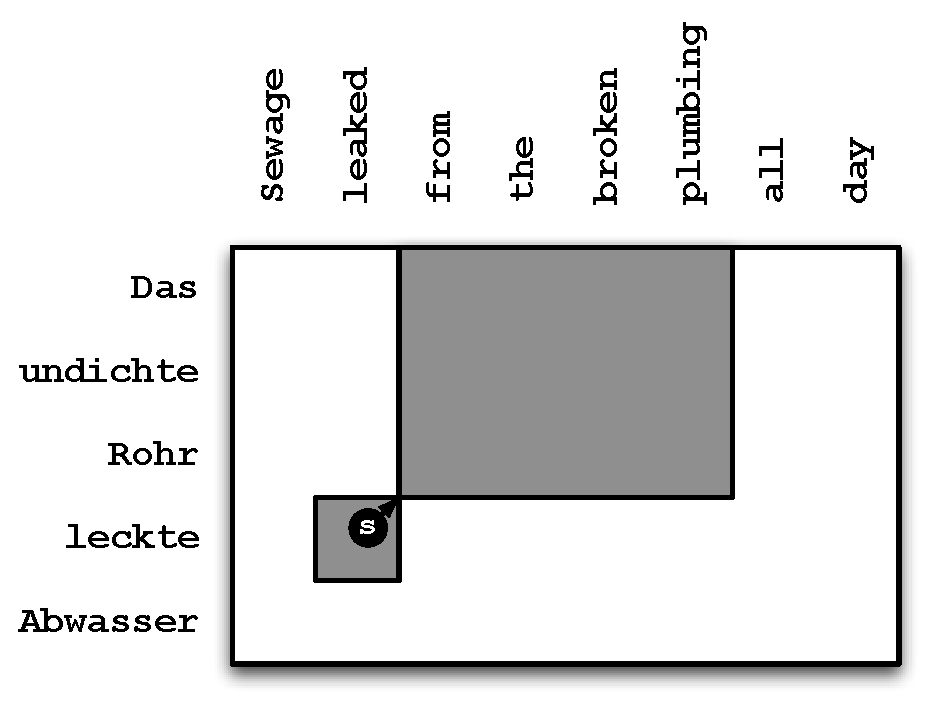
\includegraphics[width=0.8 \linewidth]{../figures/monoreord/monoreord.pdf}
\caption{Collecting phrase ordering statistics for a de-en phrase pair (\emq{leckte}, \emq{leaked}).  The longest preceding phrase \emq{Das undichte Rohr} in source, has a phrase table translation \emq{from the broken plumbing} appearing after the target phrase.}
\label{fig:monoreord}
\end{center}
\vskip -0.2in
\end{figure}

\SetAlFnt{\relsize{-1.5}}

\begin{algorithm}[t]

 \SetKwFunction{CollectOccurs}{CollectOccurs}
 \SetKwBlock{Body}{}{}
 \SetCommentSty{text}
 \SetFuncSty{text}

 \hrule \vskip 0.2cm

  \KwIn{Source and target phrases $f$ and $e$,\\
  \hskip 0.85cm Source and target monolingual corpora $\emph{C}_f$ and $\emph{C}_e$,\\
  \hskip 0.85cm Phrase table pairs $\emph{T} = \{(f^{(i)}, e^{(i)})\}_{i=1}^{N}$.}
  \KwOut{Orientation features ($p_m, p_s, p_d$).}
  
  \vskip 0.2cm \hrule \vskip 0.2cm

  $S_f \leftarrow$ sentences containing $f$ in $\emph{C}_f$\;
  $S_e \leftarrow$ sentences containing $e$ in $\emph{C}_e$\;
  
  $(B_f, -, -) \leftarrow \CollectOccurs(f, \cup_{i=1}^{N} f^{(i)}, S_f)$\;
  $(B_e, A_e, D_e) \leftarrow \CollectOccurs(e, \cup_{i=1}^{N} e^{(i)}, S_e)$\;
    
  $c_m = c_s = c_d = 0$\;
  
  \vskip 0.1cm 

  \ForEach{uniques $f_b$ in $B_f$} {
    \ForEach{translation $e^{*}$ of $f_b$ in $\emph{T}$} {

      $c_m = c_m + \#_{B_e}(e^{*})$\; 
       $c_s = c_s + \#_{A_e}(e^{*})$\; 
       $c_d = c_d + \#_{D_e}(e^{*})$\; 
    }
  }
  
  $c \leftarrow c_m + c_s + c_d$;
    
  \Return{$({c_m \over c}, {c_s \over c}, {c_d \over c})$}

  \vskip 0.2cm \hrule \vskip 0.2cm

  \CollectOccurs{$r$, $R$, $S$} \Body{
   $B \leftarrow ()$; $A \leftarrow ()$; $D \leftarrow ()$\;

    \ForEach{sentence $s \in S$} {
      \ForEach{occurrence of phrase $r$ in $s$} {
        $B \leftarrow B$ + $($longest preceding and in $R)$\;
        $A \leftarrow A$ + $($longest following and in $R)$\;
        $D \leftarrow D$ + $($longest discontinuous and in $R)$\;
      }
    }
    
    \Return{($B$, $A$, $D$)}\;
  }
  
  \vskip 0.2cm \hrule \vskip 0.2cm

  \caption{Estimating reordering probabilities from monolingual data. $B$ denotes a phrase before another phrase, $A$ denotes a phrase after it, and $D$ denotes a discontinuous relation.} \label{fig:algoreorder}
  %\vskip -0.2in
\end{algorithm}

In the phrase-based SMT pipeline we reviewed in \secref{sect:bckg:smt}, phrase pair orientation statistics were collected from induced word alignments.  We keep a similar lexicalized reordering model formulation, but infer its parameters from monolingual data instead.  The orientation information for a phrase pair is collected from source and target sentences containing the two phrases as well as other hypothesized translation pairs.  Given a phrase pair ($f$, $e$), the idea is to estimate the probability that other phrases preceding $f$ will precede, follow, or be discontinuous with $e$ in target sentences when translated.  We use phrase table entries as the contextual phrases used to to estimate these orientation features for ($f$, $e$). Consider a simple example on \figref{fig:monoreord}: the phrase pair is ($f =$ \emq{leckte}, $e =$ \emq{leaked}), and a given pair of unaligned sentences also contains a phrase table entry ($f_{b} =$ \emq{Das undichte Rohr}, \emq{from the broken plumbing}).  In this example, the phrase $f_{b}$ preceding $f$ in the source sentence swaps order with $e$ in the target.  When collected these counts over large monolingual corpora, we expect the swap, monotone, and discontinuous counts to provide good estimates for the orientation features.  
%Note that multiple phrases may immediately precede $f$ and appear in the phrase table; however, we only use the longest of them to collect reordering counts.  
Shorter and more frequent phrases (e.g. punctuation) are more likely to appear in multiple orientations with a given phrase.  Thus, we collect the longest contextual phrases (which also appear in the phrase table) for reordering feature estimation.

The algorithm on \figref{fig:algoreorder} estimates monotone, swap, and discontinuous orientation features $(p_m, p_s, p_d)$ for a phrase pair ($f, e$).  It begins by calling {\tt \small CollectOccurs()} to collect the longest matching phrase table phrases ($B_f$) preceding $f$ in source monolingual data, as well as preceding ($B_e$), following ($A_e$), and discontinuous ($D_e$) phrases with $e$ in the target language data.  For each unique phrase $f_{b}$ preceding $f$, translations are then looked up in the phrase table $\emph{T}$.  Next, we count\footnote{$\#_{L}(x)$ returns the count of object x in list L.} how many translations $e^*$ of $f_b$ appeared before, after or were discontinuous with $e$ in the target language data.  Finally, the counts are normalized and returned. \mtodo{Be more specific about the out-of-order counts?}  %The algorithm requires a single pass through the data to collect contextual phrases for the entire phrase table and its running time is quadratic in the size of the table.\mtodo{Check}

\subsection{Extracting a phrase table without a bitext}  \label{sect:extract}
We propose three methods for assembling a table of phrase translations without using parallel data. In the first, we extend past efforts in bilingual lexicon induction from monolingual corpora to the induction of multi-word phrases. In the second, we build a table of phrase pair translations from an existing bilingual seed dictionary. Finally, we use a bilingual lexicon induction framework to induce new translations for words not in our dictionary. In Section \ref{sect:exp:pt} we perform end-to-end MT experiments to test the quality of these phrase tables both individually and combined.

\paraheader{Phrase table induction.} As we argued in \secref{sect:bckg:lexind}, we cannot directly extend translation lexicon induction techniques to induce phrasal translations.  Because this search space is very large, we must aggressively prune it.   Specifically, we compare phrases in the same frequency bands \cite{Uszkoreit:2010}, require that the stemmed version of each phrase-pair contain at least one word-pair from a stemmed version of our bilingual dictionary\footnote{Our stemmer simply outputs the the first six characters of a word if it is at least six characters long, and the entire word otherwise}, and prune all very low frequency target phrases. %\todo{Alt wording:} We compare  each source side phrase only to target side phrases that occur in the same frequency band (according to the frequencies in two monolingual corpora). Of those target side phrases, we keep only the ones with at least one \mtodo{discuss dictionary parameters} word translating into a word in the source side phrase. 

To determine whether our pruning parameters are reasonable, we evaluate what percent of the items from a bilingually induced phrase table are retained.  Rather than consider all items from the phrase table (since many of them are bad), we consider only those phrase-pairs that are used by the decoder when translating a test set.\footnote{To determine which phrase pairs are used by the decoder, we use the Moses decoder's trace function to find the set of phrases used in decoding our test set} We compare our filtered phrase tables to this set of phrase translation rules and attempt to maintain as many of them as possible, while pruning the set of phrase pairs down to manageable size.

\paraheader{Dictionary-based phrase table.}\mtodo{Chris had a citation for this method} We build a second phrase table by enumerating all combinations of all translations of each word in a given source side phrase and then producing all word order permutations. Our available \mtodo{citation from this? it's a combination of some of David's dictionaries, I think} Spanish--English dictionary has over 300,000 entries and the resulting phrase table has a large amount of overlap with the decoder table, as shown in Table \ref{table:prune}. However, for the case of low-resource languages, dictionaries, in the cases that they even exist, are not as complete. We expect the performance of our dictionary-based phrase table to be an upper bound for the performance of an induced-dictionary-composed table for truly low-resource languages.

\paraheader{Induced lexical translations.} We use a bilingual lexical induction framework that works by comparing context, time, and edit distance source and target word vectors to build a table of candidate translations for those approximately ten thousand word types in our development and test sets that do not have entries in our bilingual dictionary. In Section \ref{sect:exp:pt} we use this relatively small set of unigram translation pairs to supplement the above tables.

%Our baseline phrase table is generated using a bilingual dictionary. For each Urdu test set phrase up to length three, we generated English phrases from all combinations of dictionary translations and all possible reorderings. For the baseline and our pruning methods, the number of filtered phrase pairs and the percent of phrases used by the Moses decoder not pruned away are given in Table \ref{table:prune}.  

\begin{table}
\small
\begin{center}
\begin{tabular}{|c|c|c|c|c|}
\hline
Pruning 	& Phrase	& Search & 	Findable 	& Findable \\
filters	& Pairs	&  Space & Types 	&  Tokens \\
\hline
Unpruned & 1.6 T & 100\% & 100\% & 100\% \\
Dict permut. & 74 M & $<$.01\% & 38\% & 65\% \\
Frequency &  31 B & 2\% & 75\% & 81\% \\
Freq + Dict & 566 M & $<$.04\% & 49\% & 55\% \\
\hline
\end{tabular}
\caption{This shows the tradeoff between pruning the phrase pair search space and the accuracy of the final set of phrase pairs. The findable types and tokens measures refer to the percent of phrase types and tokens used by Moses to decode a test set that are not pruned away. }\label{table:prune}
\end{center}
\end{table}

%Second round of pruning: after monolingual feature extraction, before re-ordering estimation. \todo{Needs to be discussed after explanation of those methods?}

% ------------------------------------------------

\section{Experiments} \label{sect:exp}

We used two Spanish-English corpora to estimate monolingual features: (1) in most of our experiments, we use the Spanish-English subset of the Europarl version 5 corpus \cite{Koehn:2005}; however, we treat the two sides of the corpus as two {\em independent monolingual} corpora, and (2)  Spanish and English texts (106 and 187 million tokens, respectively) annotated with publication dates we collected by crawling news sites\footnote{We have been collecting similar resources for a number of low density languages, and we plan to make them available to the community.}.

We use the Moses SMT toolkit\mtodo{Add a moses citation} and a language model trained on the English side of Europarl.  With the exception of maximum phrase length (set to 3 in our experiments\mtodo{Add the phrase length vs. performance curve?}), default values were used for all of the parameters.  We also prune the preceding, following, and discontinues phrases collected by {\tt \small CollectOccurs()} (see \figref{fig:algoreorder}) to contain at most 1,000, 1,000, and 3,000 least frequent phrases phrases, respectively.

We begin with a series of lesion experiments in which we drop feature functions estimated from parallel data.  We then add equivalent but monolingually estimated features in reverse order to see how much of the lost performance can be regained.  Finally, we move on to phrase table induction experiments.

\subsection{Dropping features}  \label{sect:exp:lesions}

We begin with a series of experiments where we remove individual features derived from an aligned bitext in order to get a sense of their relative contributions to the overall system performance on the English-Spanish language pair (see \figref{fig:lesionreplacement}).  When both phrase and orientation features are derived from word alignments ({\bf A.A}, the standard features functions defined in \secref{sect:bckg:smt}), the system reaches 21.87 BLEU.  Next we replace orientation features with random values ({\bf A.--}) and drop phrase features ({\bf --.A}).  While phrase table features account for a substantial performance difference (9 BLEU points), dropping orientation features affects the system score relatively little.  This is not surprising, since the word order is generally preserved in Spanish to English translations.  Finally, both dropping phrase scores and replacing orientation features with random values ({\bf --.--}) results in 5.5 BLEU, a 16.4 point drop.

\subsection{Adding equivalent monolingual features} \label{sect:exp:replacement}

Next, we replace the feature functions with their monolingual equivalents, hoping to regain much of the 16.4 BLEU point loss that resulted from dropping all features.  Adding orientation features estimated from monolingual data ({\bf --.M}) alone recovers 5 BLEU points. Adding phrasal monolingual scores ({\bf P.--}) and lexical monolingual scores ({\bf L.--}) separately recovers 8.4 and 10.6 BLEU points, respectively, and 11 points together. Like the phrase table features derived from the bitext, our monolingual features contribute more to performance than the reordering feature, which, as mentioned, is not surprising for Spanish to English translation. Supplementing the stripped phrase table with all three monolingually estimated features ({\bf PL.M}) yields an even higher gain of 11.6 BLEU points, or over 70\% of the BLEU score loss that occurred when we dropped all features from the phrase table. From these results, we are able to conclude that our monolingual features in combination with our orientation feature successfully recover much of the information contained in the features derived from bitext. 

We perform an additional experiment to determine whether there is any information estimated in monolingual scores that is not captured by the standard feature set derived from the bitext. Indeed, we see over a BLEU point increase when we supplement the original phrase table with phrasal and lexical monolingual features ({\bf APL.A}). Therefore, remarkably, our monolingually estimated scores capture some novel information not contained in the standard feature set.

In a final experiment, instead of estimating the monolingual scores from two sides of a parallel corpus, an idealized case, we use truly monolingual data from web crawls. In this experiment, we estimate phrasal monolingual scores, lexical monolingual scores, and orientation features all from the crawled data and achieve 13.49 BLEU on the same Spanish to English test set. This is comparable to the 17.08 BLEU achieved when using the same feature set and estimating scores using parallel data. So, although there is a significant drop in performance when we move to using strictly monolingual corpora, performance is much higher than including no phrase table features at all. In the future we plan to perform additional experiments to explore how to best take advantage of truly monolingual resources.

 Note that the BLEU score for the monolingually estimated features is equivalent to training a standard bilingually estimated system using a parallel corpus with X sentence pairs.  \mtodo{Fill in from learning curve.}

\begin{figure*}[t]
%\vskip 0.1in
\begin{center}
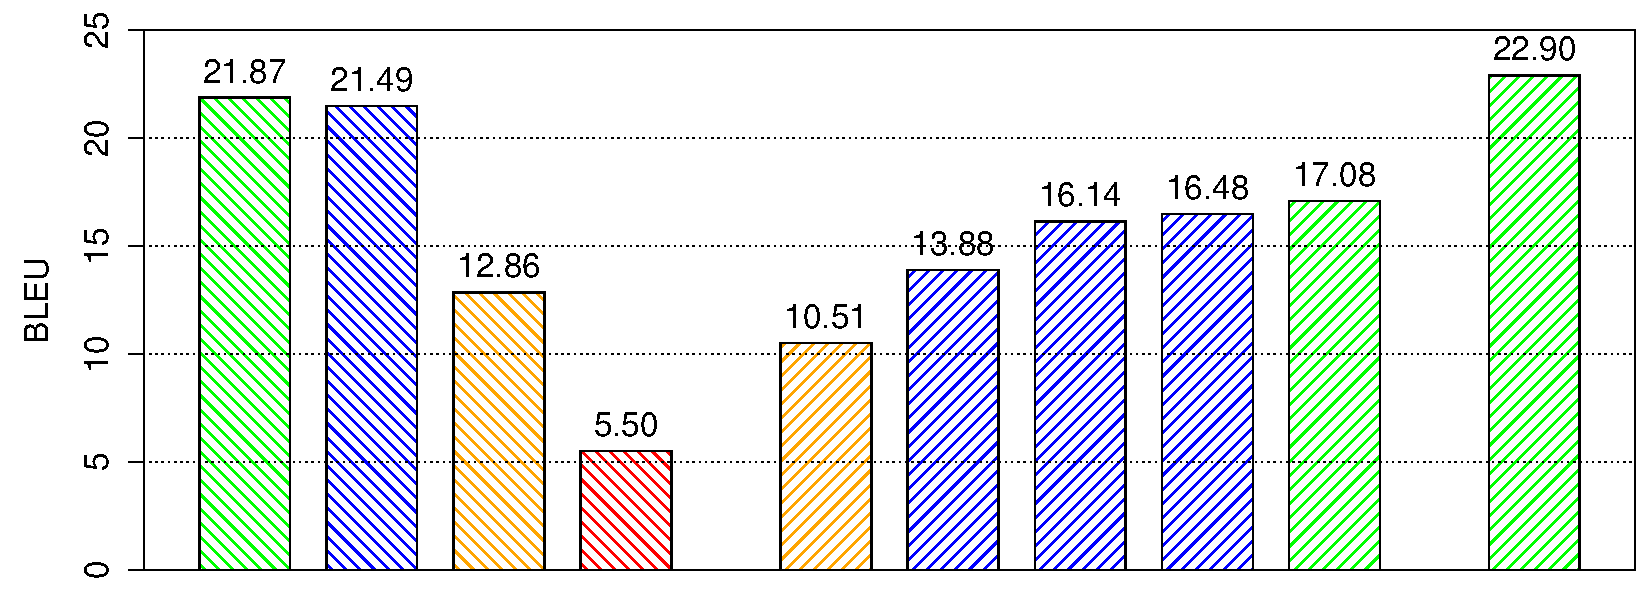
\includegraphics[width=\linewidth]{../figures/lesionreplacement/lesionreplacement.pdf}
\caption{Contributions of individual features to overall system performance: both phrase and orientation features derived from word alignments ({\bf A.A}), orientation features replaced with random values ({\bf A.--}), dropped phrase features ({\bf --.A}), and dropped phrase features and random orientations ({\bf --.--}).  Contributions due to adding back equivalent monolingual features: orientation features estimated from monolingual data ({\bf --.M}).  Random reordering features are then used with with phrasal ({\bf P.--}), and lexical monolingual scores ({\bf L.--}), as well as both ({\bf PL.--}).  ({\bf PL.M}) combines all monolingual features.  Finally, just adding phrasal and lexical monolingual similarity scores ({\bf APL.A}) substantially improves on the standard feature set ({\bf A.A}).}
\label{fig:lesionreplacement}
\end{center}
\vskip -0.2in
\end{figure*}

%\begin{figure}[t]
%%\vskip 0.1in
%\begin{center}
%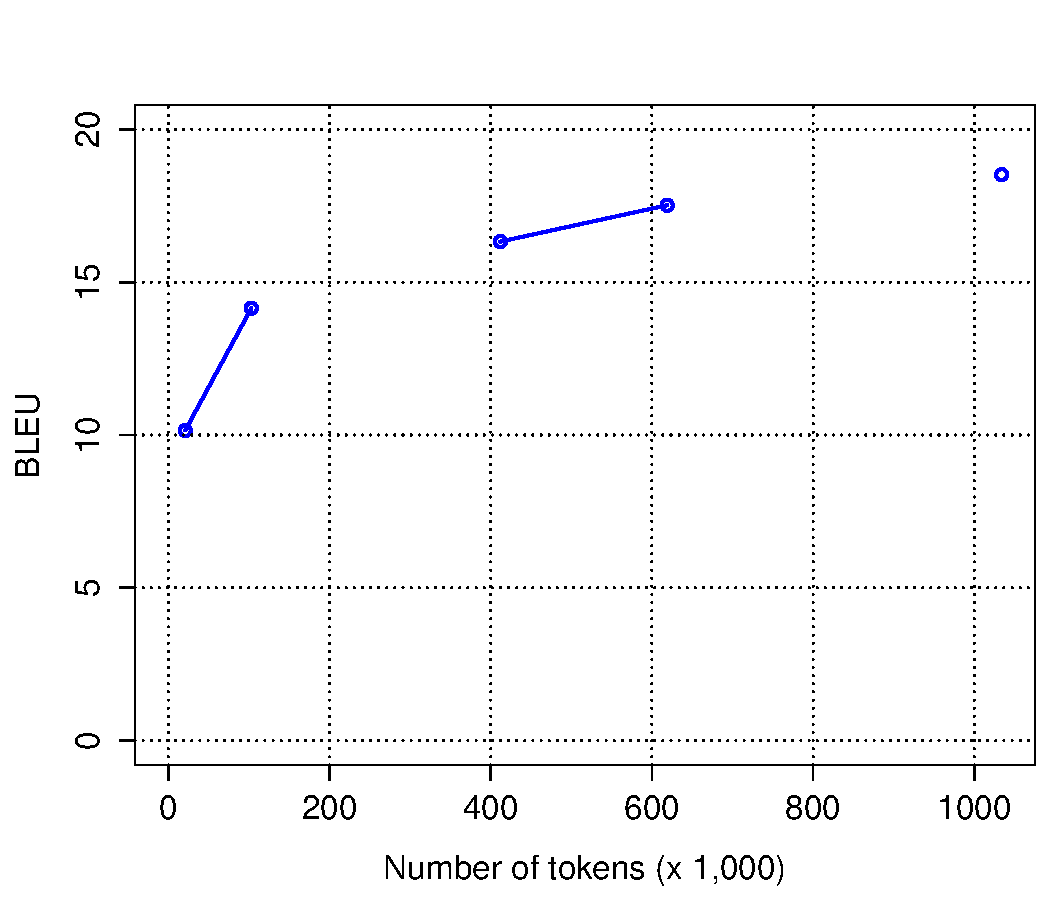
\includegraphics[width=\linewidth]{../figures/learning/learning.pdf}
%\caption{Performance of the Moses pipeline ({\bf A.A}) vs. the size of the training data (20 thousand though 1 million tokens of the Spanish-English Europarl).}
%\label{fig:learning}
%\end{center}
%\vskip -0.2in
%\end{figure}

\subsection{Phrase table extraction}\label{sect:exp:pt}
As alternatives to using the Moses phrase table, which is based on the word-aligned parallel corpus, we perform several experiments using phrase tables generated in other ways. As explained in Section \ref{sect:extract}, we generate phrase translation pairs in three ways: combining and permuting dictionary translations (henceforth, dictionary-based); using lexicon induction methods to identify candidate word translations for OOV unigrams (henceforth, lexically induced); and inducing multi-word translations from the bilingual text treated as monolingual corpora (henceforth, induced phrase pairs). We compute both lexical and phrasal monolingual feature scores for all three types of phrase translations. To score lexical monolingual features, we use the word alignments inherent to both the dictionary-based translations and the lexically induced translations. We use the Berkeley aligner \cite{DeNero07} to generate alignments for the induced phrase pairs. 

We use the monolingual feature scores to prune the induced phrase pairs from over 500 million phrase pairs to 1.1 million and to prune the dictionary-based table from 74 million to about 500 thousand entries. We include the top five lexically induced translations for each OOV unigram.

BLEU scores resulting from using different combinations of phrase pair sets and features are shown in Figure \ref{fig:phrasetable}. In all experiments using phrase pairs from multiple sources, we add a feature to indicate whether a given phrase pair came from the dictionary-based or lexically induced tables or from the large table of induced phrase pairs. As shown, using the dictionary-based table without monolingual features and using the induced phrase pairs (with features) both result in relatively poor translation performance. However, adding monolingual features to the dictionary-based table improves the BLEU score to 
11.52, and combining the dictionary-based table with the induced phrase pairs further improves the BLEU score to 12.25. Finally, combining all three alternative phrase pair sources results in a surprisingly competitive BLEU score of 12.65\mtodo{get final score with tuning, and with other lower frequency terms}. 

Although our alternative phrase pair sources do not reach the performance level of the Moses phrase table, they do show that it is possible to perform end-to-end MT without a sentence-aligned parallel corpus. We believe that this is a promising direction for future work.

\begin{figure}[h]
%\vskip 0.1in
\begin{center}
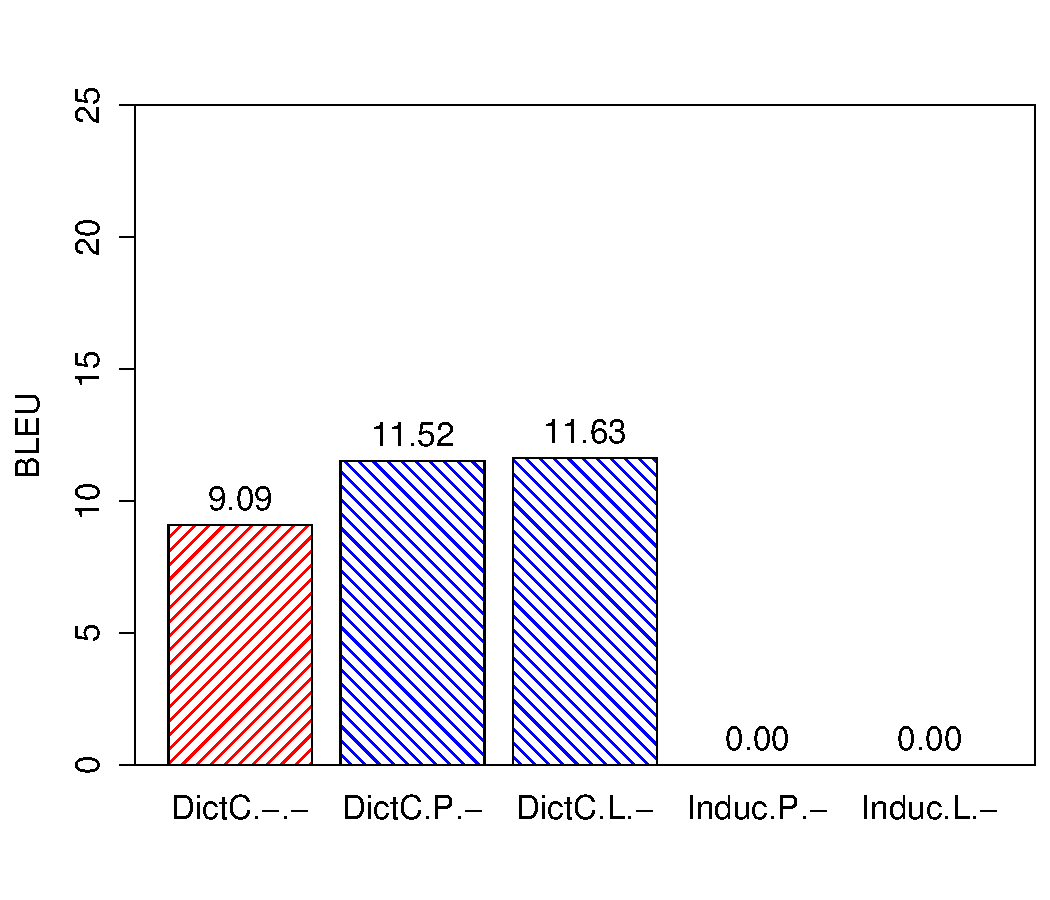
\includegraphics[width=\linewidth]{../figures/phrasetable/phrasetable.pdf}
\caption{MT performance using extracted phrase tables: dictionary-based table with no features ({\bf 1}), dictionary-based tables with phrasal monolingual scores ({\bf 2}), induced phrase pairs with monolingual features ({\bf 3}), combined dictionary-based table and induced phrase pairs with lexical and phrasal monolingual scores ({\bf 4}), and combined dictionary-based, lexically induced, and induced phrase pairs with lexical and phrasal monolingual scores ({\bf 5}). }
\label{fig:phrasetable}
\end{center}
\vskip -0.2in
\end{figure}


%\begin{table}
%\small
%\begin{center}
%\begin{tabular}{|c|c|c|c|}
%\hline
%Phrase 	& Monolinual	& Reordering & 	BLEU \\
%Table	& Features	&  Features &  \\
%\hline
%Dict-composed & None & Random & 9.09 \\
%Dict-composed & Mono & Random & 11.52 \\
%Dict-composed & Align-Mono & Random & 11.63 \\
%Induced & Mono & Random & X \\
%Induced & Align-Mono & Random & If-time \\
%\hline
%\end{tabular}
%\caption{Decoding with induced and dictionary-composed phrase tables}\label{table:new-phrase-tables}
%\end{center}
%\end{table}



%\subsection{Single language}

%\begin{enumerate}
%\item {\em Phrase features}.  (a) Augment phrase scores with mono features.  If we see better performance, reduce the amount of parallel data until it matches the performance of the original system.  Make the tradeoff argument.  (b) ({\bf lesion experiments}) See how well we do with mono features alone.
%\item {\em Orientation features}. Use mono orientation features.
%\item {\em Induce phrase table}.
%\item {\em Put everything together}.  Run the entire pipeline.
%\end{enumerate}

%\subsection{Big experiment}

%Now, run the entire pipeline on a handful of languages extracting monolingual features from the Gigaword and our crawls.

% ------------------------------------------------

% \section{Discussion} \label{sect:disc}

% ------------------------------------------------

\section{Conclusions and Future Work} \label{sect:conc}

In the future we plan to build complete systems for low resource languages. In the case that very little or no parallel text is available, we expect to significantly outperform state-of-the-art MT. We have been actively collecting newswire data for many languages, which we will use to build phrase tables and estimate monolingual features, and we will make this available to the research community.

In moving from Spanish--English translation to translation from other, less-similar languages, we expect to face new challenges. Estimating orientation probabilities, for example, for languages with very different grammars may demand a more sophisticated algorithm. However, our work here lays the foundation for this important future work.

In this paper we have made use of plentiful monolingual data to perform machine translation, which paves the way for MT systems to reduce dependence on expensive parallel data.  In particular, we have demonstrated that monolingual features on phrase translations are informative enough on their own to be used in a competitive system. In addition to monolingual feature estimates similar to those used for bilingual lexicon induction, we proposed an algorithm for estimating orientation probabilities from monolingual data. Finally, we have proposed methods for generating phrase translation pairs from monolingual data, which replace the phrase table derived from aligned parallel sentences.

In addition to proving to be competitive in {\it replacing} elements of the standard phrase-based MT pipeline, we have shown that using features derived from monolingual data to {\it augment} MT systems significantly improves performance. Simply adding our monolingual features to the phrase table results in over a BLEU point performance increase.


%\begin{itemize}
%\item Show that simply adding mono features => over a BLEU point gain.
%\item We plan to run this on real data for low resource languages.  We are have been actively collecting newswire data, which we plan to make available to the community.
%\item Language pairs with different writing system: use transliteration for edit distance features (as suggested in \secref{sect:phrasalfeats}).
%\item Showed that augmenting standard pipeline with monolingual features helps.
%\item Demonstrated that monolingual features are informative enough on their own for a competitive system.
%\item Proposed an algorithm for estimating orientation probabilities from monolingual data alone.
%\item Build complete systems for X low-resource languages.
%\end{itemize}

%\section*{Acknowledgments}
%The authors would like each other and their parents.

\newpage
\bibliographystyle{acl}
% you bib file should really go here 
\bibliography{lowresmt}

\end{document}
